
%(BEGIN_QUESTION)
% Copyright 2014, Tony R. Kuphaldt, released under the Creative Commons Attribution License (v 1.0)
% This means you may do almost anything with this work of mine, so long as you give me proper credit

Følgende trefase transformator-kobling kalles en {\it open-delta}:

$$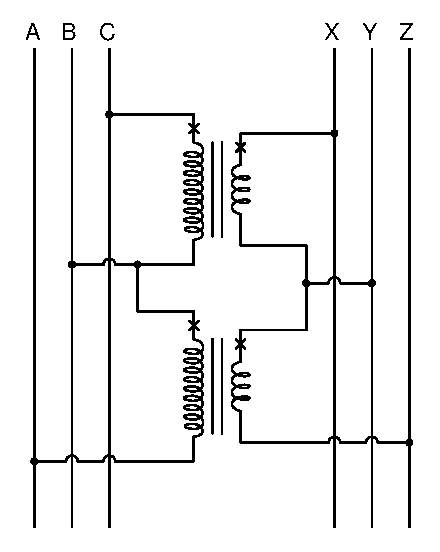
\includegraphics[width=15.5cm]{i00838x01.eps}$$

Skisser et fasordiagram som viser $V_X$, $V_Y$ og $V_Z$ med antatt 4:1 nedtransformering i hver transformator, {\it ACB}-fasefølge og $V_A$ = 277 volt $\angle$ $0^o$.

$$
\includegraphics[width=15.5cm]{i00838x02.eps}$$

\underbar{file i00838}
%(END_QUESTION)





%(BEGIN_ANSWER)

Først tegnes et fasordiagram for primærspenningene. $V_A$, $V_B$ og $V_C$ er 277 volt hver, mens $V_{BA}$ og $V_{CB}$ er 480 volt hver:

$$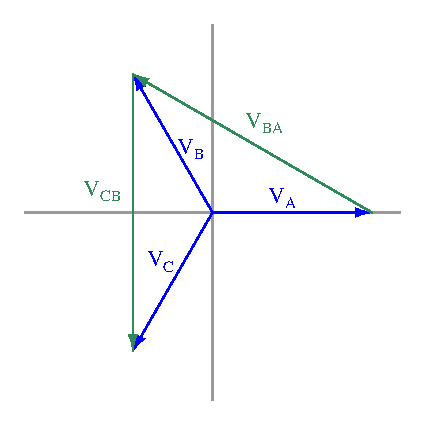
\includegraphics[width=15.5cm]{i00838x03.eps}$$

Med 480 volt over hver primærvikling får sekundærviklingene 120 volt hver (4:1-forhold). Med samme fasevinkler og samme koblingsmønster på sekundærsiden som på primærsiden, blir sekundærens fasordiagram svært likt primærens, men med en fjerdedel av fasorlengdene. Fasorene $V_{YZ}$ og $V_{XY}$ blir 120 volt hver, mens $V_X$, $V_Y$ og $V_Z$ blir 69.3 volt hver:

$$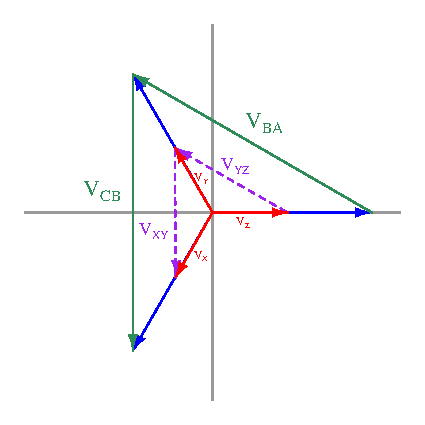
\includegraphics[width=15.5cm]{i00838x04.eps}$$

Sekundær fasefølge blir XYZ.

%(END_ANSWER)





%(BEGIN_NOTES)


%INDEX% Electronics review, 3-phase transformer bank phase shift calculations

%(END_NOTES)
